\documentclass{article}

% Language setting
% Replace `english' with e.g. `spanish' to change the document language
\usepackage[english]{babel}

% Set page size and margins
% Replace `letterpaper' with`a4paper' for UK/EU standard size
\usepackage[letterpaper,top=2cm,bottom=2cm,left=3cm,right=3cm,marginparwidth=1.75cm]{geometry}

% Useful packages
\usepackage{amsmath}
\usepackage{graphicx}
\usepackage[colorlinks=true, allcolors=blue]{hyperref}

\title{Skyedge: Empowering the Data Economy through Blockchain and Decentralized Finance}
\author{\href{https://www.dipankar.name}{\hspace{1mm}Dipankar Sarkar} \\
  \texttt{dipankar@cryptuon.com} \\
        \and
	Shaleen Mathur \\
	%% Address \\
	\texttt{shaleen@knowlcom.com} \\
	%% \And
	%% Coauthor \\
	%% Affiliation \\
	%% Address \\
	%% \texttt{email} \\
	%% \And
	%% Coauthor \\
	%% Affiliation \\
	%% Address \\
	%% \texttt{email} \\
 }
\begin{document}
\maketitle

\begin{abstract}
This white paper introduces Skyedge, a groundbreaking platform designed to revolutionize the data economy by integrating data monetization with decentralized finance (DeFi) and blockchain technology. Skyedge empowers individual users to take control of their personal data, offering a secure and transparent mechanism for data monetization, while providing businesses with access to legitimate consent-based data. By leveraging a unique multifunctional node system and an innovative tokenomics model with its native \$SKYE tokens, Skyedge aims to foster a new ecosystem where data is not only a source of insight, but also an asset class in DeFi. This document delves into Skyedge's technical architecture, market positioning, regulatory considerations, and the economic incentives designed to engage consumers, businesses, and investors in a collaborative, value-driven data economy. Through Skyedge, we envision a future where data sovereignty is the norm, businesses engage in ethical data practices, and investors contribute to a sustainable and equitable digital marketplace.
\end{abstract}

\pagebreak

\tableofcontents

\pagebreak

\section{Introduction}
In an era where data is ubiquitously hailed as the new oil, the dynamics of data generation, collection, and monetization have increasingly become central to the discourse on digital rights, privacy, and economic equity. The burgeoning digital economy, while offering unprecedented opportunities for innovation and growth, has concurrently engendered a landscape where the vast majority of generated data—particularly that which is derived from individual users—becomes the purview of a few dominant corporations. This concentration of data ownership and control not only raises profound privacy concerns but also significantly limits the potential for equitable economic participation by individual data producers. Skyedge emerges as a pioneering solution in this context, aiming to democratize data ownership and monetization through a decentralized, permissioned, and anonymized framework.

The inception of Skyedge is predicated on a critical examination of the existing data economy, which predominantly benefits large corporations that harness user-generated data without providing commensurate value to the data producers themselves. This model of data exploitation is increasingly viewed as untenable, prompting a reevaluation of how data is valued, exchanged, and controlled. Skyedge addresses this paradigm with a novel architectural approach that empowers everyday computer users, enabling them to assert control over their data and engage in its monetization within a secure, transparent, and user-centric ecosystem.

The strategic vision of Skyedge is twofold: firstly, to facilitate a shift in the power dynamics of the data economy, allowing end users to become active participants rather than passive subjects of data commodification; and secondly, to integrate consumer data into the DeFi infrastructure, thereby expanding the utility and value proposition of decentralized finance. By doing so, Skyedge not only champions individual data sovereignty but also catalyzes the convergence of data economy and DeFi, engendering a more inclusive, dynamic, and equitable digital financial landscape.

\begin{table}[h!]
\centering
\begin{tabular}{|p{2cm}|p{4.5cm}|p{4.5cm}|}
\hline
\textbf{Stakeholder} & \textbf{Before Skyedge} & \textbf{After Skyedge} \\
\hline
Consumers & Lacked control over their personal data with minimal or no compensation for its use. & Gain full control and monetization capabilities over their own data, ensuring privacy and profit. \\
\hline
Businesses & Relied on centralized data brokers, facing challenges in data authenticity and consumer trust. & Access to a decentralized marketplace for authentic, consent-based data, enhancing trust and efficiency. \\
\hline
Investors & Focused on established data and tech markets with traditional financial assets and centralized operations. & Opportunity to invest in a pioneering decentralized platform with a new asset class (data) in DeFi, promising growth and innovation. \\
\hline
\end{tabular}
\caption{Market Transformation due to Skyedge}
\label{tab:market_transformation}
\end{table}


Moreover, Skyedge is not merely a platform; it is a holistic ecosystem designed to accommodate various stakeholders, including individual users, data consumers (enterprises), and network participants (node operators). This ecosystem is underpinned by a sophisticated technical architecture that leverages blockchain technology to ensure decentralization, security, and transparency. The incorporation of consumer data into DeFi, facilitated by Skyedge, promises to broaden the horizons of what is achievable within decentralized finance, opening up new avenues for innovation, value creation, and economic empowerment.

Additionally, Skyedge envisages a future where its infrastructure supports decentralized AI, thereby contributing to the advancement of AI technologies while adhering to principles of decentralization, privacy, and user consent. This integration signifies a forward-looking approach to leveraging blockchain and AI synergies, envisioning a decentralized AI landscape that is ethical, transparent, and driven by community engagement.

In this white paper, we delineate the foundational principles, technical architecture, operational mechanics, and strategic vision of Skyedge. Our objective is to provide a comprehensive understanding of Skyedge's role as a transformative force in the data economy, its operational dynamics within the DeFi ecosystem, and its potential to underpin a new paradigm for decentralized AI. As we navigate through the subsequent sections, we invite readers to explore the intricate design and innovative features of Skyedge, a platform that stands at the vanguard of redefining data sovereignty and economic participation in the digital age.

\pagebreak

\section{Technical Overview}

The Skyedge platform is envisaged as an innovative venture into the fusion of data sovereignty, decentralized finance, and artificial intelligence, all anchored by a complex and robust technical structure. This structure is carefully crafted to not only maintain the principles of decentralization and privacy but also to enable a smooth, secure, and effective environment for the trade and monetization of data. 

At its core, the technical structure of Skyedge encapsulates a progressive mindset, merging the tenets of blockchain technology with the necessities of user-focused data management and the vast possibilities of DeFi and decentralized AI. The technical structure of Skyedge is a tribute to the platform's dedication to innovation, security, and user autonomy. 

Through its advanced network layout, amalgamation with DeFi, and vision in facilitating decentralized AI, Skyedge emerges as a symbol of advancement in the sphere of digital rights and data economy, set to transform the norms of data ownership and monetization in the digital era.


\subsection{Core Components}

\paragraph{Consumer Mobile Application} The Skyedge mobile application serves as the primary interface for end-users, a conduit through which they exercise autonomy over their data. This application is engineered to be both intuitive and secure, offering users comprehensive control over their data preferences, access rights, and monetization options. Within this application resides a sophisticated wallet mechanism, designed to store symmetric encryption keys and manage transactions within the Skyedge ecosystem. Moreover, the application is imbued with the capability to independently mine data from the user's handset, subject to stringent permission protocols, thereby ensuring that user consent is paramount.

\paragraph{Application SDK} A pivotal component of the Skyedge architecture is its Application Software Development Kit (SDK), which facilitates the creation of new, smart contract-based wallets. These wallets can be seamlessly integrated and linked back to the user's primary Skyedge wallet, establishing a secure and transparent lineage of data ownership and control. The SDK is instrumental in generating encryption keys for data blocks, thereby ensuring that each piece of data is securely encrypted and traceable to its origin. Furthermore, the SDK enables token transactions on the blockchain, using the public key encryption paradigm to safeguard the exchange and storage of data keys within the network.

\subsection{Network Architecture}

\begin{figure}[h]
    \centering
    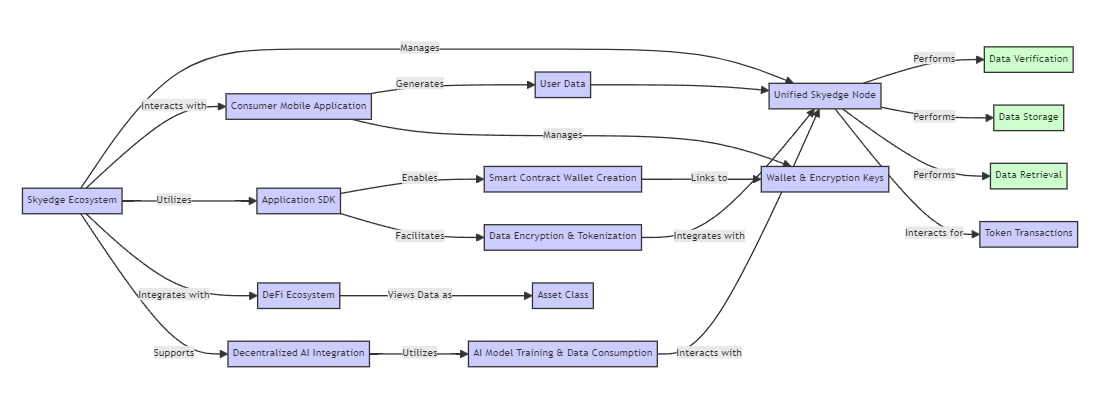
\includegraphics[width=1\linewidth]{skyedge-01.png}
    \caption{Network Architecture}
    \label{fig:network-architecturel}
\end{figure}

At the core of Skyedge's technical blueprint is its innovative network architecture, which eschews traditional centralized models in favor of a decentralized, Layer 2 solution. This choice is strategic and aims to optimize scalability, reduce transaction costs, and improve overall network efficiency. By leveraging an existing Layer 2 framework, Skyedge positions itself within the broader blockchain ecosystem, benefiting from established security protocols and network efficiencies while focusing its innovations on data monetization and user empowerment.

\paragraph{Skyedge Node} The cornerstone of Skyedge's network architecture is its unified node system. Unlike conventional blockchain networks that may deploy disparate nodes for various functions, Skyedge adopts a holistic node design where each node is capable of performing multiple functions, including data verification, storage, and retrieval. This multifunctional node architecture not only streamlines the network's operation, but also amplifies its robustness and agility. The Skyedge network nodes are incentivized through a dynamic reward mechanism, which is intricately linked to their performance in data verification, the integrity of data storage, and the efficiency of data retrieval processes.

\paragraph{Integration with DeFi and Decentralized AI}
A distinctive aspect of Skyedge's technical architecture is its profound integration with the DeFi ecosystem. By making consumer data a tradable asset within DeFi, Skyedge not only enhances the utility and liquidity of data as an asset class but also fosters a more inclusive and equitable economic model for data monetization. This integration is designed to be seamless, with smart contracts that facilitate secure and transparent exchange of data for value.

Moreover, Skyedge's architecture lays the groundwork for a decentralized AI infrastructure. By providing a platform where AI models can access diverse real-world data in a privacy-preserving and consent-based manner, Skyedge accelerates the evolution of AI in a direction that is decentralized, ethical, and community-driven. This convergence of blockchain, DeFi, and AI within Skyedge's architecture is not merely a technical achievement; it is a visionary stride towards a future where technology is leveraged for greater equity, autonomy, and innovation.

\begin{figure}[h]
    \centering
    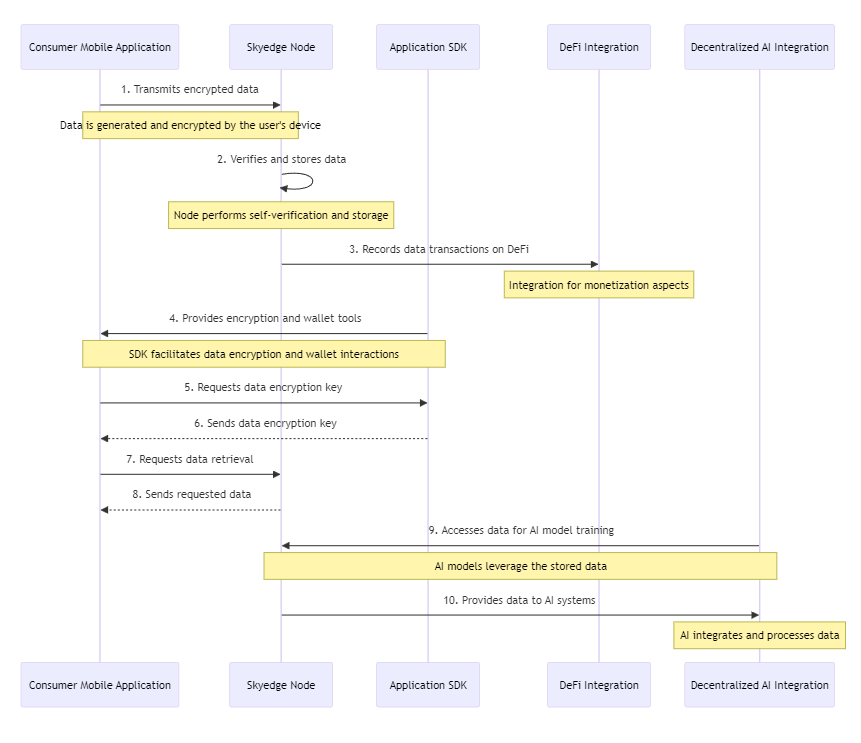
\includegraphics[width=1\linewidth]{skyedge-02.png}
    \caption{Integrations - Defi, AI}
    \label{fig:integration}
\end{figure}

\subsection{Skyedge node penalties}
In maintaining the integrity and trustworthiness of the Skyedge network, it is imperative to have a robust system in place to deter and penalize node misbehavior. The penalty mechanism is designed to ensure that all node operators adhere to the highest standards of network participation, securing the network and safeguarding user data.

\begin{itemize}
    \item \textbf{Slashing Conditions: }If a node is found to be acting maliciously, such as by attempting to manipulate data verification processes, storing data incorrectly, or failing to provide data upon legitimate retrieval requests, a portion of the staked \$SKYE tokens will be slashed. For example, engaging in data manipulation might result in a 5\% slash of the staked tokens, emphasizing the critical nature of data integrity within the network.
    \item \textbf{Downtime Penalties:} To ensure high availability and reliability of the network, nodes are required to maintain a minimum uptime. If a node's downtime exceeds the acceptable threshold (e.g., 95\% uptime over a given period), a percentage of the staked tokens could be deducted as a penalty. For instance, if a node's uptime falls below 95\%, it could face a 2\% reduction in its staked amount to incentivize continuous operation and reliability.
    \item \textbf{Performance-Based Penalties:} Beyond outright malicious behavior or excessive downtime, nodes might also be penalized for suboptimal performance. This includes slow data retrieval times or inaccurate data verification. While these penalties would be less severe than those for malicious actions, they serve to encourage and maintain a high standard of service across the network. For example, consistently underperforming nodes could see a 1\% penalty applied to their staked tokens.
    \item \textbf{Graduated Penalty System:} The penalty system is designed to be graduated, meaning that the severity of the penalty correlates with the severity and frequency of the misconduct. A node's first minor offense might incur a minimal penalty, but repeated or severe infractions would trigger more significant consequences. This system is intended to provide a learning curve and an opportunity for node operators to rectify their behavior before severe penalties are applied.
    \item \textbf{Reinstatement Post-Penalty:} Nodes that have been penalized have a path to reinstatement and redemption. After a penalty has been imposed, node operators can take corrective actions to address the issues that led to the penalty. Once these actions are verified and deemed satisfactory, the node can be reinstated with full functionality, albeit with a probation period during which the node is closely monitored for compliance.
    \item \textbf{Transparent and Fair Adjudication:} All penalty proceedings are transparent and involve a clear, predefined process. This ensures that every node operator understands the potential consequences of various actions and that penalties are applied fairly and consistently across the network.
\end{itemize}

Incorporating these penalty mechanisms reinforces the Skyedge network's resilience and reliability, ensuring that all participants are aligned with the network's goal of providing a secure, efficient, and transparent data economy. These penalties not only serve as deterrents against undesirable behavior but also as tools to educate and guide node operators toward adherence to the network's high standards, thus fostering a robust and trustworthy ecosystem.


\pagebreak

\section{Tokenomics}
The Skyedge platform has launched its proprietary token, \$SKYE, which serves as the vital force of its ecosystem, managing transactions, rewarding participants, and guaranteeing the strength and safety of its decentralized network. Taking cues from successful ERC-20 tokens, the tokenomics of Skyedge is engineered to cultivate a prosperous and enduring economy, supporting the platform's operations and providing value to its users. The tokenomics architecture is meticulously designed to promote participation, safeguard the network, and enable the smooth transfer and monetization of data. 

In essence, the tokenomics model of Skyedge is aimed at establishing a harmonious, enduring, and incentivizing economic landscape. By coordinating the interests of various stakeholders through staking prerequisites, yield models, and the tactical use of \$SKYE tokens, Skyedge strives to construct a resilient and flourishing ecosystem that backs its ambitious goals in the domains of data sovereignty, DeFi, and decentralized AI.


\subsection{Token Distribution and Allocation}
The total supply of \$SKYE tokens is meticulously capped to prevent inflation and ensure value preservation. The distribution of \$SKYE is segmented into several key allocations, reflecting the platform's priorities and strategic objectives:

\begin{itemize}
    \item \textbf{Network Incentives:} A significant portion of the total \$SKYE supply is allocated to network incentives, rewarding nodes for their roles in verification, storage, and data retrieval. This allocation is designed to ensure the ongoing participation and commitment of node operators.
    \item  \textbf{Community and Ecosystem Development:} To foster growth and engagement, a dedicated allocation is reserved for community rewards, ecosystem partnerships, and developmental initiatives, facilitating broader adoption and collaborative growth.
    \item \textbf{Team and Advisors:} A reserved percentage of \$SKYE tokens is allocated to the team and advisors, vested over a period to align their interests with the long-term success of the platform.
    \item \textbf{Reserve Fund:} A strategic reserve is maintained to provide liquidity, support platform stability, and address unforeseen contingencies, ensuring the platform's resilience.
\end{itemize}

\subsection{Staking and Node Operation}
Skyedge introduces a staking mechanism where participants can operate a node by locking a predetermined amount of \$SKYE tokens. This staking serves multiple purposes: it secures the network by ensuring the commitment of node operators, aligns incentives, and facilitates a decentralized governance model.

\paragraph{Unified Node Staking Requirement} Each Skyedge node, being multifunctional, requires a substantial staking commitment to ensure that operators are invested in the network's integrity and performance. For instance, operating a Skyedge node might require staking 10,000 \$SKYE tokens, a figure determined to balance accessibility with a meaningful commitment to the network's health.

\subsection{Yield Models}
The yield model for Skyedge node operators is designed to reward contributions to the network, with yields determined by the node's performance across its various functions:
\begin{itemize}
    \item \textbf{Verification Yield:} Nodes are rewarded for accurately verifying data integrity and authenticity, with higher rewards for consistent performance and reliability. For example, a node might receive a yield of 2\% annually for its verification activities.
    \item \textbf{Storage Yield:} Nodes are also incentivized for storing data securely and efficiently, with yields proportional to the amount of data stored and the duration of storage. A node could earn a 1.5\% yield for its storage capabilities.
    \item \textbf{Data Retrieval Yield:} Whenever a node facilitates the retrieval of data, it earns a yield. This yield is variable, depending on the frequency and volume of data retrieval requests a node processes, potentially adding an additional 1\% to 2\% yield.

\end{itemize}

\subsection{Transaction and Usage Fees}

Skyedge utilizes \$SKYE tokens for transaction fees within the network, ensuring a consistent demand for the token. These fees are used to compensate nodes for their computational efforts and to support network maintenance. Additionally, enterprises and users engaging in data transactions on the platform will use \$SKYE, further integrating the token into the platform's core activities and value exchanges.


\pagebreak

\section{Market Analysis}

The rapidly expanding digital data environment, in conjunction with the swift advancement of blockchain technology and decentralized finance (DeFi), offers a rich platform for the implementation and acceptance of Skyedge. This market analysis explores the prevailing trends, possible hurdles, and opportunities within the data economy, blockchain, and DeFi sectors, offering a thorough synopsis of the milieu in which Skyedge functions. 

The market analysis highlights the considerable potential and advantageous positioning of Skyedge within the swiftly changing digital terrain. By addressing present market demands and trends while foreseeing future progressions, Skyedge is set to establish a unique and valuable position in the data economy, blockchain, and DeFi sectors.

\begin{table}[h!]
\centering
\begin{tabular}{|p{2cm}|p{3cm}|p{3cm}|p{3cm}|p{3cm}|}
\hline
\textbf{Sector} & \textbf{Market Size} & \textbf{Growth Potential} & \textbf{Key Players} & \textbf{Emerging Trends}\\
\hline
Digital Data Economy & Estimated \$300 billion by 2025 & High growth with increasing data generation and usage & Google, Facebook, Amazon, Acxiom & Increased focus on privacy and personal data marketplaces \\
\hline
Blockchain Technology & Expected to reach \$39.7 billion by 2025 & Steady growth as adoption increases across sectors & IBM, Oracle, Deloitte, Chainalysis & Expansion beyond cryptocurrencies to supply chain, healthcare, etc.\\
\hline
Decentralized Finance (DeFi) & Over \$80 billion in total value locked & Rapid expansion with innovation in financial products & Uniswap, MakerDAO, Compound, Aave & Integration with traditional finance, regulatory adaptation\\
\hline
\end{tabular}
\caption{Market Analysis Overview for Skyedge}
\label{tab:market_analysis}
\end{table}


\subsection{Digital Data Economy}

\paragraph{Current Trends:} The global digital data sphere is expanding exponentially, with an estimated 2.5 quintillion bytes of data produced by humans every day. Enterprises across various sectors leverage this data for insights, innovation, and competitive advantage. However, the centralization of data ownership and monetization by tech conglomerates has sparked significant privacy concerns and calls for a more equitable data economy.

\paragraph{Opportunities:} Skyedge capitalizes on the growing awareness and demand for data privacy and ownership. By enabling individuals to monetize their data directly, Skyedge aligns with the trend towards greater data sovereignty and personal data control, offering a decentralized alternative to the current centralized models.

\paragraph{Challenges: }The main challenges include overcoming entrenched data monetization practices of large corporations and addressing the scalability and data security concerns inherent in handling vast amounts of personal data.

\subsection{Blockchain and Cryptocurrency Market}

\paragraph{Current Trends:} The blockchain technology market is witnessing robust growth, with increasing adoption across various sectors beyond just finance, including supply chain, healthcare, and real estate. Cryptocurrencies and tokens continue to gain traction as both investment vehicles and functional tools within blockchain ecosystems.

\paragraph{Opportunities:} Skyedge's blockchain-based architecture positions it at the forefront of this growth, offering a secure, transparent, and efficient platform for data transactions. The use of \$SKYE tokens within its ecosystem aligns with the increasing acceptance of cryptocurrency and provides a practical utility case, enhancing user engagement and network value.

\paragraph{Challenges:} The blockchain sector's rapid evolution also brings challenges, including regulatory uncertainties, high competition, and the need for continuous technological advancement to ensure security, scalability, and user-friendliness.

\subsection{Decentralized Finance (DeFi)}

\paragraph{Current Trends:} DeFi has emerged as a revolutionary force in finance, offering decentralized lending, borrowing, and trading solutions that challenge traditional financial institutions. The total value locked in DeFi protocols has soared, reflecting growing user trust and adoption.

\paragraph{Opportunities:} Skyedge's integration with DeFi through the monetization of consumer data presents a novel use case, expanding the scope of DeFi beyond purely financial assets to include data as an asset class. This not only broadens the appeal of Skyedge but also contributes to the diversification and maturation of the DeFi ecosystem.

\paragraph{Challenges:} The DeFi landscape is still nascent and volatile, with risks such as smart contract vulnerabilities, fluctuating market conditions, and regulatory scrutiny. Ensuring robust security measures and compliance with evolving regulations will be crucial for Skyedge's sustained success in this space.

\subsection{Competitive Landscape}

\paragraph{Direct Competitors:} While there may be other platforms aiming to monetize personal data or integrate blockchain with data transactions, Skyedge's unique value proposition lies in its comprehensive approach, combining data monetization with DeFi and decentralized AI.

\paragraph{Indirect Competitors:} Broader blockchain and DeFi platforms could be considered indirect competitors, though Skyedge's specific focus on data creates a niche market positioning.

\paragraph{Differentiation:} Skyedge differentiates itself through its multifaceted node ecosystem, robust tokenomics, and the integration of data assets into the DeFi space, appealing to a broad audience ranging from individual data producers to enterprise data consumers and blockchain enthusiasts.


\pagebreak

\section{Regulatory and Legal Considerations}
In developing and deploying a groundbreaking platform like Skyedge, which intersects the realms of data monetization, blockchain, and decentralized finance (DeFi), meticulous attention to the regulatory and legal landscape is paramount. This section elucidates the various regulatory frameworks and legal considerations that Skyedge navigates to ensure compliance, foster trust, and uphold its commitment to legal integrity and user protection.

The regulatory and legal considerations for Skyedge are multifaceted and central to its design and operation. Ensuring compliance with data protection laws, financial regulations, and IP rights, while effectively navigating the complex web of jurisdictional variances, is crucial for Skyedge's legitimacy, user trust, and long-term success. By proactively addressing these considerations, Skyedge aims to establish a robust, compliant, and ethically-grounded platform at the forefront of the data economy and blockchain innovation.

\subsection{Data Protection and Privacy Laws}

\paragraph{Global Data Privacy Regulations:} Skyedge operates in a domain where data is the primary asset, necessitating stringent adherence to international data protection laws such as the General Data Protection Regulation (GDPR) in the European Union, the California Consumer Privacy Act (CCPA), and other jurisdiction-specific regulations. Compliance with these laws requires robust data handling and processing protocols, ensuring user consent, data minimization, and the right to data erasure are strictly observed.

\paragraph{Anonymization and Consent:} Skyedge's architecture is designed to anonymize user data and requires explicit user consent for data sharing and transactions, aligning with legal standards for personal data protection. The platform must continuously adapt to evolving data protection laws and ensure that user empowerment and privacy are at the forefront of its operational ethos.

\subsection{Blockchain and Cryptocurrency Regulations}

\paragraph{Compliance with Financial Regulations:} As Skyedge integrates DeFi elements and utilizes its native \$SKYE tokens within its ecosystem, compliance with financial regulations, including anti-money laundering (AML) and know your customer (KYC) frameworks, becomes crucial. Skyedge must navigate the regulatory variances across jurisdictions, particularly focusing on the classification of \$SKYE tokens (whether as securities, commodities, or otherwise) and adhering to relevant financial oversight mechanisms.

\paragraph{Token Sale and Securities Laws:} The initial offering and distribution of \$SKYE tokens must be meticulously planned to comply with securities laws globally. This involves determining whether the tokens constitute securities under various jurisdictions and ensuring that the token sale process adheres to legal requirements, avoiding the pitfalls that have ensnared numerous blockchain ventures.

\subsection{Jurisdictional Considerations}

\paragraph{Navigating Multiple Jurisdictions:} Given the global nature of blockchain and data markets, Skyedge must be adept at operating within the legal frameworks of multiple jurisdictions, each with its own regulations governing data protection, blockchain technology, and financial transactions. Strategic decisions regarding the domiciliation of Skyedge entities and the choice of jurisdictions for operation will significantly impact regulatory compliance and business operations.

\paragraph{Smart Contract Disputes:} As Skyedge leverages smart contracts for data transactions and node operations, establishing a clear legal framework for resolving disputes related to smart contract executions is essential. This includes defining the jurisdiction and applicable law in smart contract terms, ensuring clarity and enforceability.

\pagebreak

\section{Risk Analysis}
The introduction of Skyedge as a pioneering platform at the intersection of data monetization, decentralized finance (DeFi), and blockchain technology embodies a transformative step forward but also entails a spectrum of risks. This risk analysis section employs a game-theoretic approach to dissect potential risks, considering the strategic interactions between various stakeholders and the systemic implications of those interactions. By anticipating and strategizing against potential adversarial behaviors and systemic vulnerabilities, Skyedge aims to fortify its infrastructure and ecosystem against foreseeable challenges.

By adopting a game-theoretic perspective, Skyedge can anticipate and strategize against various adversarial and systemic risks. This approach allows for the design of mechanisms and incentives that align stakeholders' interests with the platform's long-term viability and success, fostering a resilient and robust ecosystem in the face of uncertainties and adversarial pressures.

\subsection{Technological Risks}

The core operations of Skyedge rely on smart contracts. There is an inherent risk of vulnerabilities or bugs, which malicious actors could exploit, potentially leading to loss of funds or data breaches. Game-theoretic analysis suggests that as the value locked in Skyedge's contracts increases, so does the incentive for attackers to exploit these contracts. Regular audits and employing a bug bounty program are strategic defenses against this risk.

Given the data-centric nature of Skyedge, there is a critical risk associated with data leakage or breaches. In a game where adversaries gain from acquiring data without consent, Skyedge must ensure robust encryption and anonymization techniques, minimizing the payoff for potential attackers and increasing the cost of malicious endeavors.

\subsection{Market Risks}

The \$SKYE token's value may be subject to high volatility, influenced by market dynamics, overall crypto market trends, and investor sentiment. Stakeholders, particularly node operators, may engage in speculative behavior, affecting network stability. Game theory suggests that designing staking mechanisms and tokenomics with anti-speculative measures can mitigate such risks, aligning incentives towards long-term network health.

The success of Skyedge is partially contingent on achieving a critical mass of users and node operators, creating a network effect. There's a coordination game at play where individuals' readiness to join the platform depends on others' participation. Early and consistent incentives for early adopters and a robust marketing strategy can help overcome initial inertia, catalyzing the network effect.

\subsection{Regulatory Risks}
The rapidly evolving regulatory landscape for blockchain and data monetization poses a significant risk. Changes in regulations could impact Skyedge's operations, particularly in jurisdictions with stringent data privacy and blockchain regulations. Here, a game of cat-and-mouse unfolds where regulators set rules and platforms adapt, necessitating a proactive and adaptive legal strategy from Skyedge to stay compliant while pursuing its objectives.

As Skyedge operates across various jurisdictions, the risk of non-compliance with local laws, especially concerning data privacy and financial regulations, is significant. The strategic interaction between Skyedge and regulatory bodies is akin to a signaling game, where Skyedge must continuously signal compliance and transparency to maintain legitimacy and operational freedom.

\subsection{Operational Risks}
Skyedge's performance and reliability are contingent on external infrastructures, such as Ethereum for its L2 solutions. Any disruptions or failures in these underlying technologies pose direct risks to Skyedge's operations. A strategic approach involves diversification and redundancy in external dependencies to minimize single points of failure.

The decentralization aspect introduces risks related to node misbehavior, including potential collusion or Sybil attacks. In this game, nodes have financial incentives to act honestly or maliciously, depending on the relative payoffs. Implementing rigorous staking and slashing mechanisms can alter the payoff matrix for nodes, incentivizing cooperative and honest behavior.

\pagebreak

\section{Summary}
As we culminate our exploration of the Skyedge white paper, it is imperative to underscore the transformative potential that Skyedge holds for consumers, businesses, and investors, marking a significant leap forward in the realms of data monetization, decentralized finance (DeFi), and blockchain technology. Skyedge is not merely a technological innovation; it represents a paradigm shift, a reimagining of data's role in our digital society, and a new frontier in the interplay between technology and economic empowerment.

\subsection*{For Consumers}
Skyedge heralds a new era of data sovereignty and economic agency for consumers. By enabling individuals to take control of their data and partake in its monetization, Skyedge empowers consumers to be active participants in the data economy, not merely passive sources of data. This empowerment is aligned with the growing global emphasis on data privacy and consumer rights, reflecting a future where individuals can harness their data as a valuable asset, engaging in the data economy on their own terms and with full transparency and security.

\subsection*{For Businesses}
For enterprises and data consumers, Skyedge offers a novel avenue to access authentic, consent-based data, enhancing their decision-making processes, and fostering more personalized and effective solutions. The platform's decentralized, transparent, and efficient data marketplace not only broadens businesses' access to valuable insights but also instills a new level of trust and compliance in data transactions. This is particularly pivotal in a landscape increasingly characterized by stringent data protection regulations and the imperative for ethical data practices.

\subsection*{For Investors}
Investors in the Skyedge platform are at the vanguard of a groundbreaking venture that intersects several high-growth domains: blockchain, DeFi, and data monetization. The innovative use of \$SKYE tokens within the ecosystem, backed by a robust tokenomics model, presents a compelling value proposition for investors. Moreover, by investing in Skyedge, stakeholders are contributing to a future where the digital economy is more inclusive, equitable, and aligned with the broader societal values of privacy, transparency, and user empowerment.

\paragraph{}
\paragraph{}

As we stand on the cusp of this new digital epoch, Skyedge invites consumers to reclaim their data autonomy, businesses to redefine their data practices, and investors to champion a platform that stands for innovation, integrity, and inclusivity. Together, we can forge a digital landscape where data serves as a bridge to opportunity, equity, and advancement for all.

 Skyedge is more than a platform or a product—it is a vision for the future, a testament to the potential of blockchain and decentralized technologies to catalyze real-world change. We extend our heartfelt invitation to all stakeholders to join us in this journey, to be part of a movement that values data dignity, champions economic empowerment, and paves the way for a more equitable digital future.

\pagebreak

\section{Appendix}
The Appendix serves to provide additional information, clarification, and resources that supplement the main content of the Skyedge White Paper. This section is instrumental in providing comprehensive information and supporting details to stakeholders, ensuring a thorough understanding of the Skyedge ecosystem.

\subsection{Glossary of Terms}
\paragraph{Blockchain:} A distributed ledger technology that maintains a secure and decentralized record of transactions across a network of computers.

\paragraph{Smart Contracts:} Self-executing contracts with the terms of the agreement written directly in lines of code, facilitating, verifying, or enforcing the negotiation or performance of a contract.

\paragraph{Decentralized Finance (DeFi):} An emerging financial technology based on secure distributed ledgers similar to those used by cryptocurrencies, extending the use of blockchain from simple value transfer to more complex financial use cases.

\paragraph{ERC-20:} A standard for creating and issuing smart contract-based tokens on the Ethereum blockchain.

\paragraph{Node:} A computer connected to a blockchain network, which supports the network through validation, storage, and sometimes the transmission of transactions.

\paragraph{Staking:} Participating in a Proof-of-Stake (PoS) system by holding funds in a cryptocurrency wallet to support network operations.

\paragraph{Tokenomics:} The economic principles and considerations that govern the issuance, distribution and management of a cryptocurrency or token within its ecosystem.

\paragraph{KYC (Know Your Customer):} The process of a business verifying the identity of its clients, a standard practice in the investment and financial sectors.

\paragraph{AML (Anti-Money Laundering):} Legal controls that require financial institutions and other regulated entities to prevent, detect, and report money laundering activities.


\end{document}